
\chapter{Methods}




\section{Neuron and network model}

\begin{figure}
  \centerline{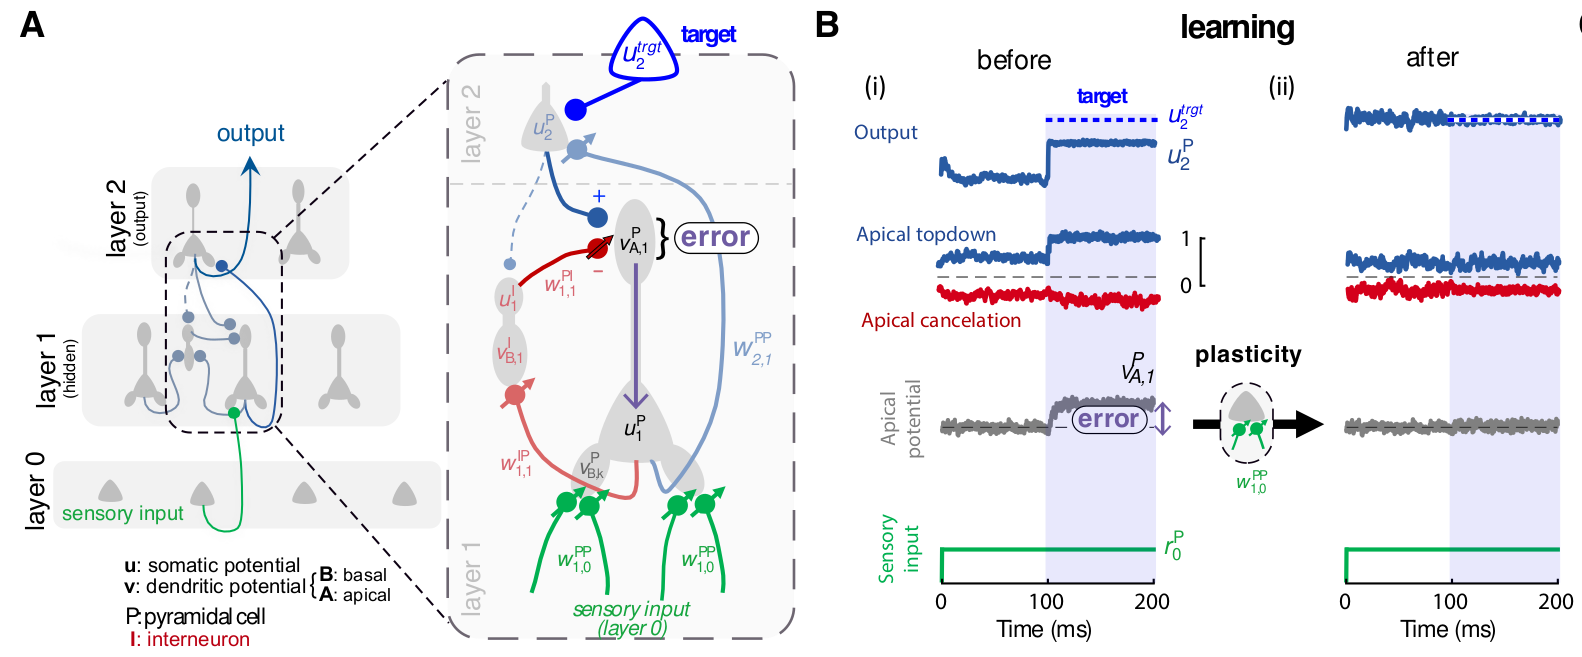
\includegraphics[width={1\linewidth}]{pyramidal.png}}
  \caption{Self-predicting initialization without plasticity}
\end{figure}
\section{Urbanczik-Senn Plasticity}


from \cite{Haider2021}:

\textit{In this architecture, plasticity serves two purposes. For pyramidal-to-pyramidal feedforward synapses,
  it implements error-correcting learning as a time-continuous approximation of BP. For pyramidal-to-
  interneuron synapses, it drives interneurons to mimic their pyramidal partners in the layers above (see
  also SI). Thus, in a well-trained network, apical compartments of pyramidal cells are at rest, reflecting
  zero error, as top-down and lateral inputs cancel out. When an output error propagates through the
  network, these two inputs can no longer cancel out and their difference represents the local error ei .
  This architecture does not rely on the transpose of the forward weight matrix, improving viability for
  implementation in distributed asynchronous systems. Here, we keep feedback weights fixed, realizing
  a variant of feedback alignment. In principle, these weights could also be learned in order to further
  improve the local representation of errors Section 7.}




One-sided exponential decay kernel

\begin{align}
  \kappa(t) & = H(t)e^{-t/\tau_{\kappa}} \\
  H(t)      & =
  \begin{cases}
    1 & \text{if $t > 0$}    \\
    0 & \text{if $t \leq 0$} \\
  \end{cases}
\end{align}

Antiderivatives:

\begin{align}
  \int_{-\infty}^x H(t)dt = tH(t) = max(0,t)
\end{align}

Convolution:

\begin{align*}
  (f \ast g)(t) & = \int_{- \infty }^{\infty} f(\tau) g(t-\tau) d \tau
\end{align*}
For functions f, g supported on only $[0, \infty]$ (as one-sided decay kernels and spiketrains are), integration limits can be truncated:
\begin{align*}
  (f \ast g)(t) & = \int_{0}^{t} f(\tau) g(t-\tau) d \tau \\
\end{align*}


Plasticity:

\begin{align}
  \frac{dW_{ij}}{dt}(t) & = F(W_{ij}(t), s_i^\ast (t), s_j^\ast (t), V_i^\ast (t)) \\
  F[s_j^\ast, V_i^\ast] & = \eta \kappa \ast (V_i^\ast s_j^\ast)                   \\
  \text{with } V_i^\ast & = (s_i - \phi(V_i )) h(V_i),                             \\
  s_j^\ast              & = \kappa_s \ast s_j.
\end{align}

For an event-based plasticity we need:

\begin{align}
  \Delta W_{ij}(t,T) & = \int_t^T dt' F[s_j^\ast , V_i^\ast ](t')                                                 \\
                     & = \int_t^T dt' \eta \kappa \ast (V_i^\ast s_j^\ast)                                        \\
                     & = \eta \int_t^T dt' \  \int_0^{t'} dt'' \ \kappa(t'-t'') V_i^\ast (t'') s_j^\ast (t'')     \\
                     & = \eta \int_0^t dt' \  \int_{t''}^{t'} dt'' \ \kappa(t'-t'') V_i^\ast (t'') s_j^\ast (t'') \\
\end{align}


Starting with the complete Integral from $t=0$.

\begin{align*}
  \Delta W_{ij}(0,t) & =\eta \int_0^t dt' \  \int_0^{t'} dt'' \ \kappa(t'-t'') V_i^\ast (t'') s_j^\ast (t'')                          \\
                     & = \eta \int_0^t dt'' \  \int_{t''}^{t} dt' \ \kappa(t'-t'') V_i^\ast (t'') s_j^\ast (t'')                      \\
                     & = \eta \int_0^t dt'' \  \left[ \tilde{\kappa}(t-t'') - \tilde{\kappa}(0) \right] V_i^\ast (t'') s_j^\ast (t'') \\
\end{align*}

With $\tilde{\kappa}$ being the antiderivative of $\kappa$:

\begin{align*}
  \kappa(t)         & = \frac{\delta}{\delta t} \tilde{\kappa}(t) \\
  \tilde{\kappa}(t) & = - e^{-\frac{t}{t_{\kappa}}}               \\
\end{align*}

The above can be split up into two separate integrals:
\begin{align*}
  \Delta W_{ij}(0,t) & =\eta \left[ -I_2 (0, t) + I_1(0,t) \right]                                      \\
  I_1(t_1, t_2)      & = - \int_{t_1}^{t_2} dt' \ \tilde{\kappa} (0) V_i^\ast (t') s_j^\ast (t')        \\
  I_2(t_1, t_2)      & = - \int_{t_1}^{t_2} dt' \ \tilde{\kappa} (t_2 - t') V_i^\ast (t') s_j^\ast (t') \\
\end{align*}

Which implies the identities

\begin{align*}
  I_1(t_1, t_2 + \Delta t) & = I_1 (t_1, t_2) + I_1 (t_2, t_2 + \Delta t)                                       \\
  I_2(t_1, t_2 + \Delta t) & = e^{- \frac{t_2 - t_1}{\tau_{\kappa}}} I_2 (t_1, t_2) + I_2 (t_2, t_2 + \Delta t)
\end{align*}


\begin{align}
  I_2 (t_1, t_2 + \Delta t) & = -\int_{t_1}^{t_2 + \Delta t} dt' \ \tilde{\kappa} (t_2 + \Delta t - t') V_i^\ast (t') s_j^\ast (t')                                        \\
                            & = -\int_{t_1}^{t_2} dt' \ \left[ -e^{- \frac{t_2 + \Delta t - t'}{\tau_\kappa}} \right] V_i^\ast (t') s_j^\ast (t')
  -\int_{t_2}^{t_2 + \Delta t} dt' \ \left[ -e^{- \frac{t_2 + \Delta t - t'}{\tau_\kappa}} \right] V_i^\ast (t') s_j^\ast (t')                                             \\
                            & = -e^{- \frac{ \Delta t}{\tau_\kappa}} \int_{t_1}^{t_2} dt' \ \left[ -e^{- \frac{t_2 - t'}{\tau_\kappa}} \right] V_i^\ast (t') s_j^\ast (t')
  -\int_{t_2}^{t_2 + \Delta t} dt' \ \left[ -e^{- \frac{t_2 + \Delta t - t'}{\tau_\kappa}} \right] V_i^\ast (t') s_j^\ast (t')
\end{align}


Using this we can rewrite the weight change from $t$ to $T$ as:


\begin{align*}
  \Delta W_{ij}(t,T) & = \Delta W_{ij}(0,T) - \Delta W_{ij}(0,t)                                               \\
                     & = \eta [-I_2(0,T) + I_1(0,T) + I_2(0,t) - I_1(0,t)]                                     \\
                     & = \eta [I_1(t,T) - I_2(t,T) + I_2(0,t)\left( 1 - e^{- \frac{T-t}{\tau_\kappa}} \right)]
\end{align*}

The simplified \cite{sacramento2018dendritic} case would be:

\begin{align*}
  \frac{dW_{ij}}{dt} & = \eta (\phi(u_i) - \phi(\hat{v_i})) \phi(u_j)                                         \\
  \Delta W_{ij}(t,T) & = \int_t^T dt' \ \eta \  (\phi(u_i^{t'}) - \phi(\widehat{v_i^{t'}})) \  \phi(u_j^{t'}) \\
  \Delta W_{ij}(t,T) & = \eta \int_t^T dt' \  (\phi(u_i^{t'}) - \phi(\widehat{v_i^{t'}})) \ \phi(u_j^{t'})    \\
  V_i^*              & = \phi(u_i^{t'}) - \phi(\widehat{v_i^{t'}})                                            \\
  s_j^*              & = \kappa_s * s_j
\end{align*}


Where $s_i$ is the postsynaptic spiketrain and $V_i^*$ is the error between dendritic prediction and somatic rate and $h( u )$. The additional nonlinearity $h( u ) = \frac{d}{du} ln \  \phi(u)$ is ommited in our model \todo{should it though?}.



\begin{align}
  \tau_l & = \frac{C_m}{g_L} = 10 \\
  \tau_s & = 3
\end{align}

Writing membrane potential to history (happens at every update step of the postsynaptic neuron):

\begin{lstlisting}[language=C++, directivestyle={\color{black}}
                   emph={int,char,double,float,unsigned,exp},
                   emphstyle={\color{blue}}]

UrbanczikArchivingNode< urbanczik_parameters >::write_urbanczik_history(Time t, double V_W, int n_spikes, int comp)
{
	double V_W_star = ( ( E_L * g_L + V_W * g_D ) / ( g_D + g_L ) );
	double dPI = ( n_spikes - phi( V_W_star ) * Time::get_resolution().get_ms() )
      * h( V_W_star );
}\end{lstlisting}

I interpret this as:


\begin{align*}
  \int_{t_{ls}}^T dt' \ V_i^* & = \int_{t_{ls}}^T dt' \  (s_i - \phi(V_i )) h(V_i),               \\
  \int_{t_{ls}}^T dt' \ V_i^* & = \sum_{t=t_{ls}}^T \  (s_i(t) -  \phi(V_i^t ) \Delta t) h(V_i^t) \\
\end{align*}

\begin{lstlisting}[language=C++, directivestyle={\color{black}}
                   emph={int,char,double,float,unsigned,exp},
                   emphstyle={\color{blue}}]
for (t = t_ls; t< T; t = t + delta_t)
{
   	minus_delta_t = t_ls - t;
    minus_t_down = t - T;
    PI = ( kappa_l * exp( minus_delta_t / tau_L ) - kappa_s * exp( minus_delta_t / tau_s ) ) * V_star(t);
    PI_integral_ += PI;
    dPI_exp_integral += exp( minus_t_down / tau_Delta_ ) * PI;
}  
// I_2 (t,T) = I_2(0,t) * exp(-(T-t)/tau) + I_2(t,T)
PI_exp_integral_ = (exp((t_ls-T)/tau_Delta_) * PI_exp_integral_ + dPI_exp_integral);
W_ji = PI_integral_ - PI_exp_integral_;
W_ji = init_weight_ + W_ji * 15.0 * C_m * tau_s * eta_ / ( g_L * ( tau_L - tau_s ) );    
  
kappa_l = kappa_l * exp((t_ls - T)/tau_L) + 1.0;
kappa_s = kappa_s * exp((t_ls - T)/tau_s) + 1.0;
  \end{lstlisting}


\begin{align*}
  \int_{t_{ls}}^T dt' s_j^* & =  \tilde{\kappa_L}(t') * s_j -  \tilde{\kappa_s}(t') * s_j
\end{align*}

$I_1$ in the code is computed as a sum:

\begin{align}
  I_1 (t,T) = \sum_{t'=t}^T \ (s_L^*(t') - s_s^*(t')) * V^*(t')
\end{align}


\section{steady-state potentials in Sacramento (2018)}

\begin{align*}
  u_k^p           & = \frac{g_B}{g_{lk} + g_B + g_A} v^P_{B,k} + \frac{g_A}{g_{lk} + g_B + g_A} v^P_{A,k} \\
  \hat{v}^P_{B,k} & = \frac{g_B}{g_{lk} + g_B + g_A} v^P_{B,k}                                            \\
  \hat{v}^I_{k}   & = \frac{g_B}{g_{lk} + g_B} v^I_{k}                                                    \\
  \lambda         & = \frac{g_{som}}{g_{lk} + g_B + g_{som}}
\end{align*}


\section{Multi-compartment neuron models}

The derivative somatic membrane potential of a pyramidal neuron in layer $l$ is given by:

\begin{align*}
  C_m \dot{u}_l^P &= - g_l u_l^{som} + g^{bas} v_l^{bas} + g^{api} v_l^{api} \\
\end{align*}

where $v_i^{bas}$ and $v_i^{api}$ are the basal and apical compartment potentials respectively, and $g^{bas}$
 and 
$g^{api}$ the dendritic coupling conductances. An interneuron integrates synaptic information by the same principle, but 
instead of feedback information arriving at the apical compartment, it is integrated directly into the soma with the 
basal potential $v_l^{bas}$\footnote{Note, that \cite{Haider2021} differentiates between pyramidal neuron
conductances $g^{bas}$ and interneuron dendritic conductances $g^{dend}$. Since they share the same value in all relevant
simulations at hand, this separation has been omitted for the sake of brevity}:

\begin{align*}
  C_m \dot{u}_l^I &= - g_l u_j^{I} + g^{bas} v_j^{bas} + i^{nudge, I} \\
  i^{nudge, I} &= g^{nudge, I} u_{l+1}^P\\
\end{align*}

where $ g^{nudge, I}$ is the interneuron nudging conductance, and $u_{l+1}^P$ is the somatic voltage of a corresponding
pyramidal neuron in the next layer. \todo{discuss whether this 1 to 1 style connection is plausible!}. Pyramidal neurons
in the output layer $N$ effectively behave like interneurons, as they receive no input to their apical compartment. Instead,
the target  activation $u^{tgt}$ is injected into their soma:

\begin{align*}
  C_m \dot{u}_N^P &= - g_l u_N^{P} + g^{bas} v_N^{bas} + i^{nudge, tgt} \\
  i^{nudge, tgt} &= g^{nudge, tgt} u^{tgt}\\
\end{align*}

\todo{
  \cite{Haider2021} uses more complex differentials. maybe create a second branch to try them out? 
}


\section{Cortical microcircuits}


\section{Haider 2021 updates}

Besides the using a prediction of future somatic activity for neuronal transfer and plasticity, \cite{Haider2021} also
slightly alter the plasticity rule, which turns out to be crucial for the latent equilibrium mechanism. While the 
simulations by \cite{sacramento2018dendritic} use the equations above, the new implementation \href{https://github.com/neurips}{fill with neurips link}
implicitly change them within its code. The fundamental building block of a network here is a layer, which is 
represented in code as an instance of the class \texttt{Layer}. Each instances holds information about its corresponding 
pyramidal- and interneurons. It also holds information about the synaptic connections between the two populations, as
well as all incoming feedforward and feedback pyramidal synapses. A layer has two class methods that are fundamental 
to its computation; \texttt{update()} computes membrane potential derivatives and synaptic weight changes given pyramidal
neuron activations from the previous and subsequent layers. \texttt{apply()} updates weights and membrane potentials 
from the previously calculated changes. Layers are processed in order from input to output layer, where all of them
receive the \texttt{update()} signal first, before \texttt{apply()} is called on all of them. This ordering ensures,
that changes in activation do not cascade through the layers and lead to excessive activations at the output. Yet, 
since next layer activations at time $t$ have not been computed, top down information is always delayed by one timestep.
\todo{evaluate importance of this}


Thus, the equations for membrane updates change slightly:

\begin{align*}
  \dot{W_{ij}}(t) & = \eta (\phi(u_i) - \phi(\alpha v^{basal}_i(t))) \phi(u_j)                                         \\
  \Delta W_{ij}(t,T) & = \int_t^T dt' \ \eta \  (\phi(u_i^{t'}) - \phi(\widehat{v_i^{t'}})) \  \phi(u_j^{t'}) \\
  \Delta W_{ij}(t,T) & = \eta \int_t^T dt' \  (\phi(u_i^{t'}) - \phi(\widehat{v_i^{t'}})) \ \phi(u_j^{t'})    \\
  V_i^*              & = \phi(u_i^{t'}) - \phi(\widehat{v_i^{t'}})                                            \\
  s_j^*              & = \kappa_s * s_j
\end{align*}



\section{Latent equilibrium}

\begin{align*}
  \phi(V^{som}) & \rightarrow \phi(\breve{V}^{som}) \\
  \breve{V}     & := V + \tau^m \dot{V}             \\
\end{align*}
\begin{align*}
  \frac{d}{dt} W_{ba} & = \eta (\phi(V_b^{som}) - \phi(\alpha V_b^{dend})) \phi(V_a^{som})                         \\
  \frac{d}{dt} W_{ba} & = \eta (\phi(\breve{V}_b^{som}) - \phi(\alpha \breve{V}_b^{dend})) \phi(\breve{V}_a^{som})
\end{align*}


\section{simulation details/updates}

All voltages need to be reset between simulations!

